\documentclass[../root]{subfiles}
\graphicspath{{_images/}{../_images/}}

\begin{document}

    \chapter{Immigration Restrictions as Active Labor Market Policy: Evidence from the Mexican Bracero Exclusion}

    \begin{shortsummary}
        \begin{itemize}
            \item \authoryear{Clemens2018} 
            \item \RQ{How effects Labor scarcity on wages? }
            \item \answer{This paper use theoretical framework and Difference-in-Difference method using agriculture data when bracero exclusion is occurred.}
            \item \result{Estimation results is insignificants and Bracero exclusion don't lead to increase farmer workers' wage and employment. }
        \end{itemize}
    \end{shortsummary}

    \section{Introduction}
    Theoretical studies suggest that labor scarcity can have ambiguous effect on wage under endogenous  technological advance.
    
    A flat or even upward sloping labor demand curve,
    \begin{itemize}
        \item under models of directed technical change(Acemoglu 2007; Accemoglu and Autor 2011)
        \item under models when production technologies of differing input intensities coexist in equilibrium.(Doms, and Lewis 2010; Manuelli and Seshadri 2014)  
    \end{itemize}
    
    Authors evaluate the labor market effect of a change of  labor market policy.This policy change was the December, 1964 abrogation  bracero agreements between the United States and Mexico.  \\
    The primary goal of bracero exclusion was to improve wages and employment for domestic farm workers. \\
    This paper build a theoretical framework and estimate the policy impact to check this policy meet its goal. \\
    Bracero exclusion had insignificant effect on wage or employment for domestic farm workers, and endogenous technical advance was an important mechanism. \\
    The contribution of this paper evaluate the policy change to exclude immigrants.  \\
    Hornbeck and Naidu (2014) show that labor scarcity arising from interstate migration after flooding can induce technological advance in agriculture. But, evidence on the effect of workforce reduction thorogh international migration barriers remains scant.
     
    \section{The Exclusion of Bracero Workers}
    The bracero agreements were a bilateral agreements between the United States and Mexico to regulate bilateral flow of temporary low-skill labor, spanning the period 1942-1964.  \\
    After the WW II the program focused almost entirely on agriculture and grow to supply almost half a million seasonal workers each year to US forms.  \\
    
    Secretary of Labor (1966) claim that due to bracero exclusion "tens of thousands of jobs were created for American workers".
    US Senate(1966) claim that positive wage effect from bracero exclusion due to trends in affected states, without nothing similar trends in unaffected states.
    
    \section{Testing a Model of Workforce Reduction and Technical Advance}
    {\bf A Crop Production in an Open Economy with Alternative Technologies} \\
    We assume there are two technology economic model and consider how be the wage  determined.
    
    Each locations $i$ can produce a single crop and its price is $p\equiv 1$.
    The endowment of land are fixed at $\overline{T}$.
    Capital and material are supplied elastically.
    Land and labor market are competitive.
    Farmers rent land at rate $r_t$ and purchase materials at price $m$.
    
    A nested CES production technology using "old" $K_O$ can be used to the output crop Y:
    
    \begin{align}
        Y_O = \left\{K_O^{\frac{\mu -1}{\mu}}+\left[a L^{\frac{\sigma -1}{\sigma}}+(1-a)T^{\frac{\sigma -1}{\mu}}\right]^{\frac{\mu-1}{\mu}\frac{\sigma}{\sigma-1}} \right\}^{\frac{\mu}{\mu-1}},
    \end{align}
    where we assume the relationship land $\tau$ and material $M$ as $T \equiv\{\tau, M\}$ for simplicity. \\
    
    The same production function for "advanced" can represents as:
    \begin{align}
        Y_A = \left\{K_A^{\frac{\mu -1}{\mu}}+\left[b L^{\frac{\sigma -1}{\sigma}}+(1-b)T^{\frac{\sigma -1}{\mu}}\right]^{\frac{\mu-1}{\mu}\frac{\sigma}{\sigma-1}} \right\}^{\frac{\mu}{\mu-1}}
    \end{align}
    Advanced technology is less labor-intensive, that is $b<a$. \\
    Because it is more land intensive, the advanced technology is more productive only at low levels of labor per unit of land and does not traditional technology.\\
    
    $K_O$ is elastically supplied at rental rate $r_O$. \\
    From the F.O.C. we get $r_O= \left\{K_O^{\frac{\mu -1}{\mu}}+\left[a L^{\frac{\sigma -1}{\sigma}}+(1-a)T^{\frac{\sigma -1}{\mu}}\right]^{\frac{\mu-1}{\mu}\frac{\sigma}{\sigma-1}} \right\}^{\frac{1}{\mu-1}}K_O^{-\frac{1}{\mu}}$ . \\
    Thus $Y_O=\left(\frac{r_O^{\mu-1}}{r_O^{\mu-1}-1}\right)^{\frac{\mu}{\mu-1}} \left[a L^{\frac{\sigma -1}{\sigma}}+(1-a)T^{\frac{\sigma -1}{\sigma}}\right]^{\frac{\sigma}{\sigma-1}} $. \\
    Authors define the cone of diversification as $[\phi_l, \phi_u]$ which are the range of $\overline{L}/\overline{T}$.  \\
    At the upper end, only the older technology is used, and at the lower end only the advanced is used.When $\phi$ is between the upper end and the lower end, fixed wage $\hat{w}$ and land rental rates $\hat{t}_T$ can write as:
    \begin{align}
        \hat{w} =a\left(\frac{r_O^{\mu-1}}{r_O^{\mu-1}-1}\right)^{\frac{\mu}{\mu-1}} \left[a +(1-a)\phi_u^{-\frac{\sigma -1}{\sigma}}\right]^{\frac{\sigma}{\sigma-1}-1} 
        =b\left(\frac{r_A^{\mu-1}}{r_A^{\mu-1}-1}\right)^{\frac{\mu}{\mu-1}} \left[b +(1-b)\phi_l^{-\frac{\sigma -1}{\sigma}}\right]^{\frac{\sigma}{\sigma-1}-1} 
        \tag{A.2} \\
        \hat{r}_T=(1-a)\left(\frac{r_O^{\mu-1}}{r_O^{\mu-1}-1}\right)^{\frac{\mu}{\mu-1}} \left[a\phi_u^{\frac{\sigma -1}{\sigma}} +(1-a)\right]^{\frac{\sigma}{\sigma-1}-1} 
        =b\left(\frac{r_A^{\mu-1}}{r_A^{\mu-1}-1}\right)^{\frac{\mu}{\mu-1}} \left[b\phi_l^{\frac{\sigma -1}{\sigma}} +(1-b)\right]^{\frac{\sigma}{\sigma-1}-1}  \nonumber
    \end{align}
   Dividing first by second equation reveals that$\phi_u = (\frac{1-b}{b}\frac{a}{1-a})^{\sigma}\phi_l$.Furthermore, 
   \begin{align}
       \phi_l = (\frac{1-b}{b})^{\frac{\sigma}{\sigma-1}} \left[\frac{\left(\frac{r_A^{\mu-1}}{r_A^{\mu-1}-1}/\frac{r_O^{\mu-1}}{r_O^{\mu-1}-1} \right)^{\frac{\mu}{\mu-1}(\sigma-1)}- (\frac{1-a}{1-b})^{\sigma}}{(\frac{a}{b})^{\sigma} -\left(\frac{r_A^{\mu-1}}{r_A^{\mu-1}-1}/\frac{r_O^{\mu-1}}{r_O^{\mu-1}-1} \right)^{\frac{\mu}{\mu-1}(\sigma-1)}} \right]^{\frac{\sigma}{\sigma-1}} \tag{A.3}
   \end{align}
   The wage inside the cone can also be written as
   \begin{align}
       \hat{w} = b^{\frac{\sigma}{\sigma-1}}\left(\frac{r_A^{\mu-1}}{r_A^{\mu-1}-1}/\frac{r_O^{\mu-1}}{r_O^{\mu-1}-1} \right)^{\frac{\mu}{\mu-1}(\sigma-1)} \left[\frac{(\frac{a}{b})^{\sigma} - (\frac{1-a}{1-b})^{\sigma}}{\left(\frac{r_A^{\mu-1}}{r_A^{\mu-1}-1}/\frac{r_O^{\mu-1}}{r_O^{\mu-1}-1} \right)^{\frac{\mu}{\mu-1}(\sigma-1)}- (\frac{1-a}{1-b})^{\sigma}} \right]^{\frac{\sigma}{\sigma-1}}
   \end{align}
    Wage is dependent only land rental rate $r_O$ and $r_A$, and labor intensity $a$ and $b$ because factor proportions are fixed within each technology.  \\
    
    \begin{figure}
        \centering
        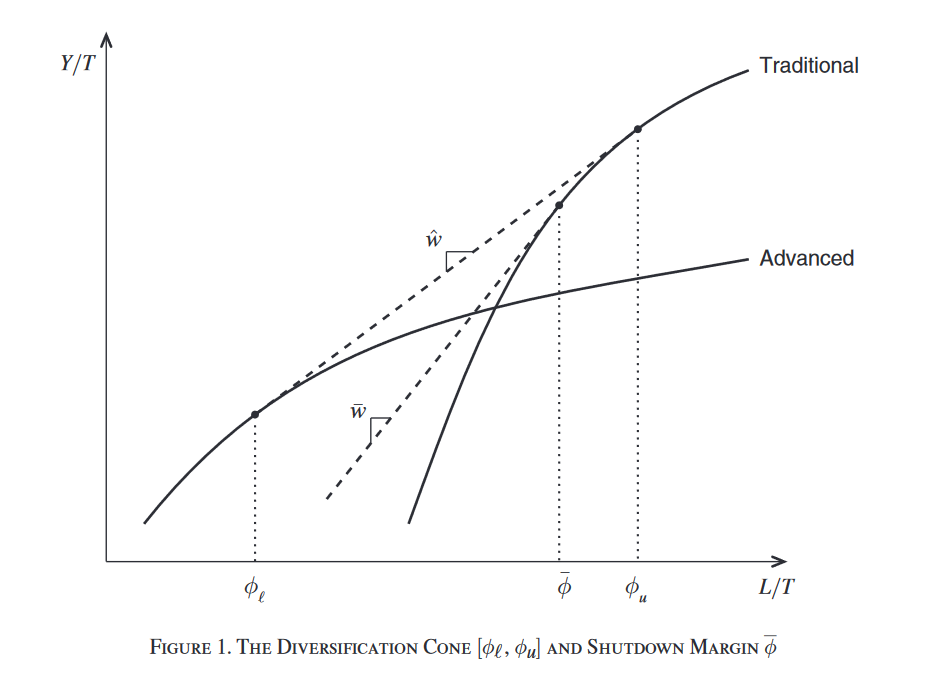
\includegraphics[width = \linewidth]{0731sugiyama/Figure1.png}
        \label{fig:my_label}
    \end{figure}

    {\bf Workforce Reduction Policy}
    
    Let consist of bracero workers $B$ and non-bracero workers $N$, such that $\overline{L} \equiv B+N$. We assume $(B+N)/ \overline{T} > \phi_l$ ; at least one farm uses the old technology.  \\
    When bracero are excluded, the relative change in labor supply is $\% \Delta (\overline{L}/\overline{T}) = \frac{N/T - (B+N)/T}{((B+N)/T)}= -\frac{B}{T}$ . 
    Using traditional technology, the wage is given by the  $w=a\left\{(\frac{K}{T})^{\frac{\mu-1}{\mu}}+\Tilde{L}^{\frac{\sigma}{\sigma-1}\frac{\mu-1}{\mu}} \right\}^{\frac{\mu}{\mu-1}-1}\Tilde{L}^{\frac{\sigma}{\sigma-1}\frac{\mu-1}{\mu}-1}(\frac{L}{T})^{-\frac{1}{\sigma}} $, \\
    where $\tilde{L}= a(\frac{L}{T})^{\frac{\sigma-1}{\sigma}} +(1-a)$.
    
    We consider three cases:
    \begin{enumerate}
        \item In the absence of adjustment in capital, technology, or output.
        \item Only capital adjustments work
        \item With Adjustment of Capital, Technology, and Output.
    \end{enumerate}
    If first case is occurred, exclusion raises wages. \\
    We define income share of land, labor, and capital as $s_T, s_L, \mbox{and} \ s_K$;
    \begin{align*}
        s_K&= \frac{r_O K_O}{Y_O} = \left\{K_O^{\frac{\mu -1}{\mu}}+\left[a L^{\frac{\sigma -1}{\sigma}}+(1-a)T^{\frac{\sigma -1}{\mu}}\right]^{\frac{\mu-1}{\mu}\frac{\sigma}{\sigma-1}} \right\}^{-1} K_O^{\frac{\mu-1}{\mu}} \\
        1-s_K&=  \left\{K_O^{\frac{\mu -1}{\mu}}+\left[a L^{\frac{\sigma -1}{\sigma}}+(1-a)T^{\frac{\sigma -1}{\mu}}\right]^{\frac{\mu-1}{\mu}\frac{\sigma}{\sigma-1}} \right\}^{-1}\left[a L^{\frac{\sigma -1}{\sigma}}+(1-a)T^{\frac{\sigma -1}{\mu}}\right]^{\frac{\mu-1}{\mu}\frac{\sigma}{\sigma-1}} \\
        s_L&=a\left\{K_O^{\frac{\mu -1}{\mu}}+\left[a L^{\frac{\sigma -1}{\sigma}}+(1-a)T^{\frac{\sigma -1}{\mu}}\right]^{\frac{\mu-1}{\mu}\frac{\sigma}{\sigma-1}} \right\}^{-1}\left[a L^{\frac{\sigma -1}{\sigma}}+(1-a)T^{\frac{\sigma -1}{\mu}}\right]^{\frac{\mu-1}{\mu}\frac{\sigma}{\sigma-1}-1} L^{\frac{\sigma-1}{\sigma}} \\
        \frac{s_L}{1-s_K}&=\left[a L^{\frac{\sigma -1}{\sigma}}+(1-a)T^{\frac{\sigma -1}{\mu}}\right]^{-1} aL^{\frac{\sigma-1}{\sigma}},
    \end{align*}
    with $s_L+s_T=1-s_K$.
    
    \begin{align}
        \frac{\partial \ ln \ w}{\partial (B/L)} \simeq \frac{\partial \ ln \  w}{\partial (L/T)} \simeq s_K\frac{s_L}{s_L+s_k}\frac{1}{\mu} + \frac{s_T}{s_L+s_K} \frac{1}{\sigma} >0
    \end{align}
    
    Using the parameter estimates of Herrendorf, Herrington, and Valentinyi(2015) for postwar US agriculture, the semi-elasticity (4) approximately 0.4.  In a typical high- bracero to state stack with $B/L=0.3$, farm wage rise by about 12 \% after exclusion. 
    
    If second case is occurred, (4) equation reduce to 
    \begin{align}
        \frac{\partial ln \ w}{\partial (B/L)} \simeq \frac{s_T}{s_L+s_T} \frac{1}{\sigma} >0
    \end{align}
    
    Where after capital adjustment,  $w =\left(\frac{r_O^{\mu-1}}{r_O^{\mu-1}-1}\right)^{\frac{\mu}{\mu-1}} \left[a(\frac{L}{T})^{\frac{\sigma-1}{\sigma}} +(1-a)\right]^{\frac{\sigma}{\sigma-1}} a(\frac{L}{T})^{-\frac{1}{\sigma}}$.
    Thus $\frac{\partial \ ln \ w}{\partial (B/L)} \simeq \frac{\partial \ ln \  w}{\partial (L/T)} \simeq -\left[\frac{1}{\sigma}\frac{s_L}{1-s_K}- \frac{1}{\sigma} \right] = \frac{s_T}{s_L+s_T}\frac{1}{\sigma}$. \\
    Under same parameter assumption, the semi-elasticity (5) is approximately 0.1, or one-quarter as large as without capital adjustment.In a typical-bracero state, exclusion raises farm wages by approximately 3 \%. \\
    If third case is occurred, the model predicts three effect of exclusion.  \\
    Assume that both the old and advanced technology are in use ($(B+N) / \overline{T} \in [\phi_l, \phi_u] $) and remain use in after exclusion ($N/ \overline{T} \in [\phi_l, \phi_u]$).First, the wage remains fixed at $w \equiv \hat{w}$ so wage do not rise:
    \begin{align}
        \frac{\partial ln \ w}{\partial (B/L)} = 0
    \end{align}
    second and third:
    \begin{align}
        \frac{\partial (Y_A/Y)}{\partial (B/L)} >0  \nonumber\\
        \frac{\partial (Y_O)}{\partial (B/L)}<0
    \end{align}
    The output share of the advanced technology rise in pre-exclusion bracero share, while the output of old technology falls.Intuitively, bracero exclusion does not affect wages within the diversification cone because any fall in the labor-land ratio only raises the fraction of farmer using the advanced technology. 
    
    {\bf Archival Data on Bracero, Farm Employment, and Farm Wages} \\
    Data on seasonal hired form workers are monthly stock of hired workers on farms by states from 1943 to 1973, with complete state coverage after 1953.Farm wage data are quarterly, with complete geographic coverage for the principal wage index 1948-1971.Sample size of the employment and wage are 10,329 and  5,813, respectively. 
    
    {\bf Data source} \\
    For the main analysis period of 1953-1973, the information published in government sources over time periods was originally gathered through a monthly farm survey conducted by the Department of Labor's state-level employment service office(DOL, 1956). \\
    All farm wage data were sourced from the Department of Agriculture publication Farm labor on a quarterly basis.  \\
    The 1950 total population of each U.S. state is form from Richard L.Forstall (1996), Population of the State and Counties of the United State: 1970 to 1990.
    
    
    \begin{figure}
        \centering
        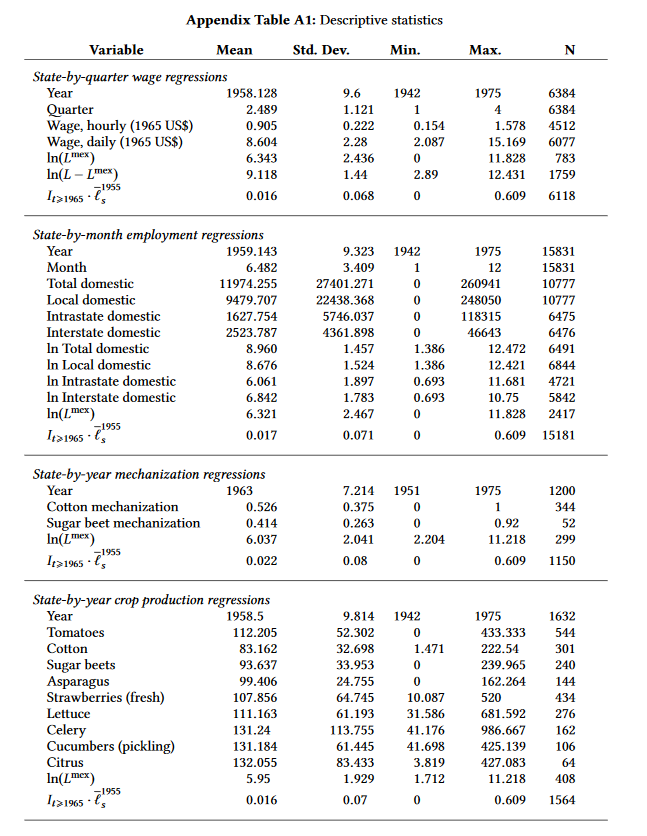
\includegraphics[width = \linewidth]{0731sugiyama/TableA1.png}
        \label{fig:my_label}
    \end{figure}
    
    \section{Results}
    
    Here authors test the model prediction that bracero exclusion could have minimal labor-market effects. \\
    {\bf Quasi-Experimental Tests: Wages and Employment} \\
    The first regression specification evaluates the effect of bracero exclusion as a quasi-experiment. Treatment is the degree of seasonal agricultural labor in the state of the program's height in the mid-1950s.Authors use Difference-in-difference with continuous treatment, follow Card(1992).
    
    \begin{align}
        y_{st}= \alpha' I_s + \beta'I_t +\gamma(I_{t \geq 1965} \cdot \overline{l}^{1955}_s) +\epsilon,
    \end{align}
    where $I_s$ is a vector of state$s$ fixed effect and $I_t$ is year, quarter, or month $t$ fixed effect. $I_{t \geq 1965}$ is an indicator for an observation after bracero exclusion. \\
    Authors use the mean of fraction Mexican workers $\overline{l}^{1955}_s$= $L^{Mex}_{st}/ L_{st}$ in state $s$. $L^{Mex}_{st}$ and $ L_{st}$ are the stock of Mexican hired seasonal workers and the stack of hired seasonal workers of any nationality, respectively. \\
    Assuming that trends in the outcome would have been similar in the most affected by exclusion to trends in unaffected stats had exclusion not occurred.

    {\bf Wages} \\
    Figure 2 illustrate the core results. Panel A show the natural experiments of bracero exclusion.States are categorize follow three states.
    begin{figure}
    \begin{figure}
        \centering
        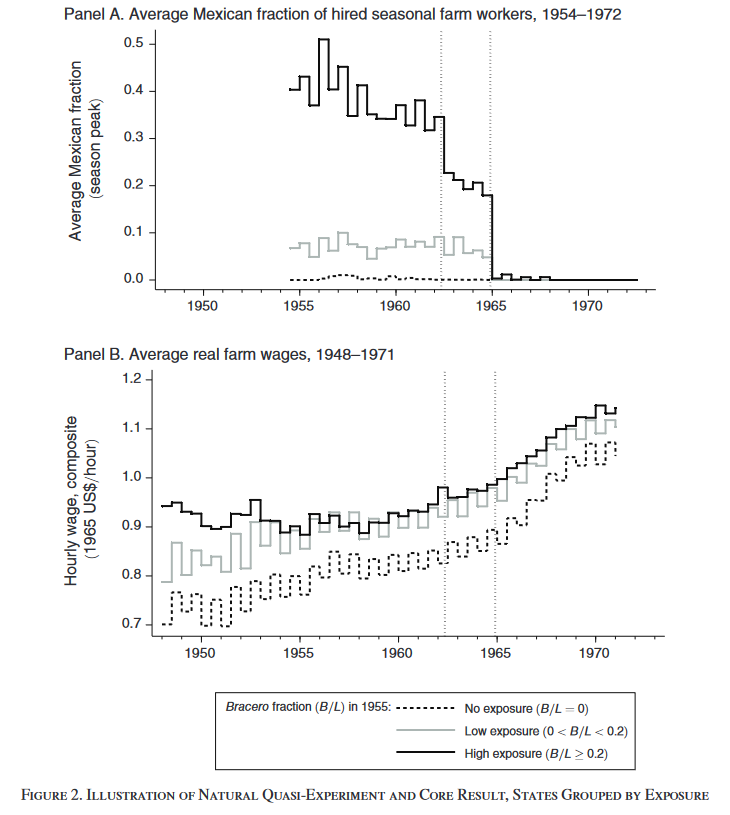
\includegraphics[width = \linewidth]{0731sugiyama/Figure2.png}
        \label{fig:my_label}
    \end{figure}
    
    \begin{description}
        \item [High exposure] Bracero made up more than 20 \% of hired seasonal farm labor in 1955. 
        \item [Low exposure]  Bracero made up less than 20 \% of hired seasonal farm labor in 1955. 
        \item [No exposure] The states had zero bracero in 1955.
    \end{description}
    Panel B show farm wage trends in the same three exclusion.Pre- and post-exclusion trends in real farm wages are similar in high-exposure states and low-exposure states.
    
    Table 1 conduct this test, using regression (8).
    \begin{figure}
        \centering
        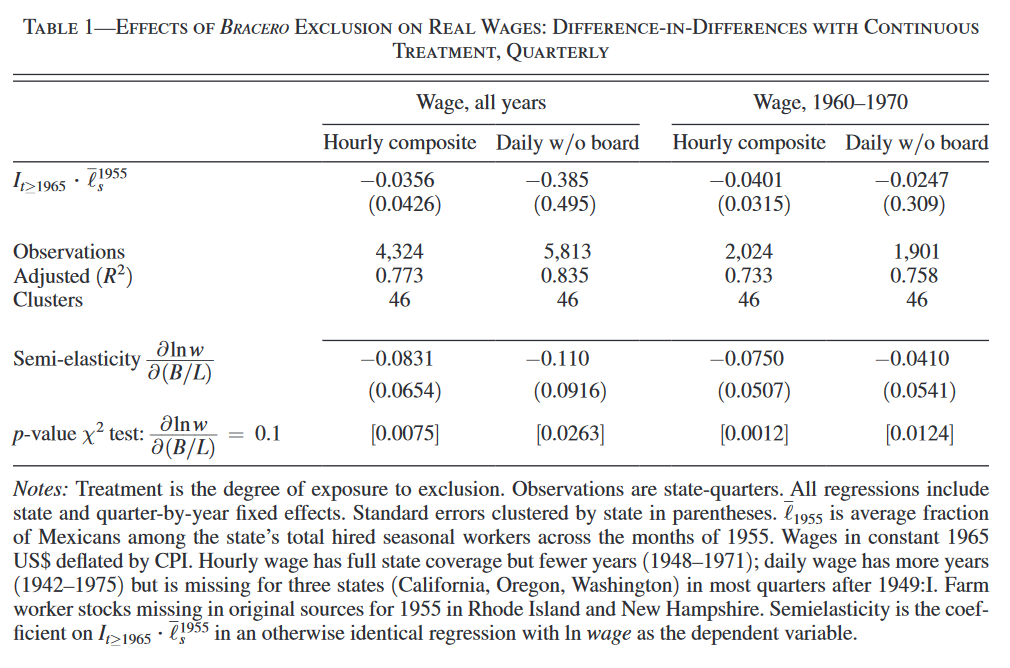
\includegraphics[width = \linewidth]{0731sugiyama/Table1.png}
        \label{fig:my_label}
    \end{figure}
    
    The first and second column use the hourly wage and the daily wage without board by state-quarter as the outcomes. The third and fourth column narrow the window of analysis to five year before and after termination of the program.  \\
    The difference-in-difference is negative but statistically distinguishable from zero. The results are compatible with rapid adjustment of capital, technology, and output in equation (6).
    
    {\bf Employment}\\
    Figure 3 illustrate core results.
    \begin{figure}
        \centering
        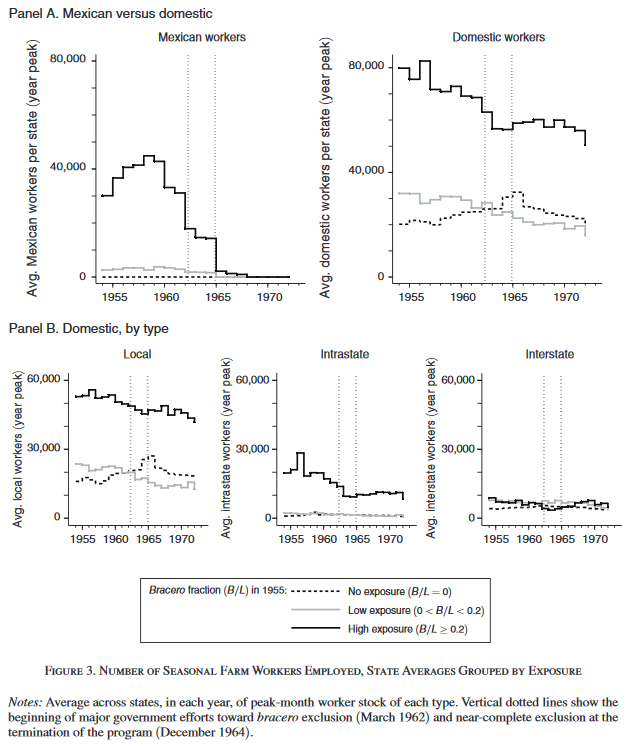
\includegraphics[width = \linewidth]{0731sugiyama/Figure3.png}
        \label{fig:my_label}
    \end{figure}
    Panel A show average bracero stock in the three groups of states over time (left).Bracero exclusion removed tens of thousands of farm workers from the average high-exposure states. \\
    It also show the average number of domestic seasonal farm workers in the same group of states(right).   The gap between high- and low- exposure states is approximately constant before and after exclusion.  \\
    Table 2 show the results of regression.
    \begin{figure}
        \centering
        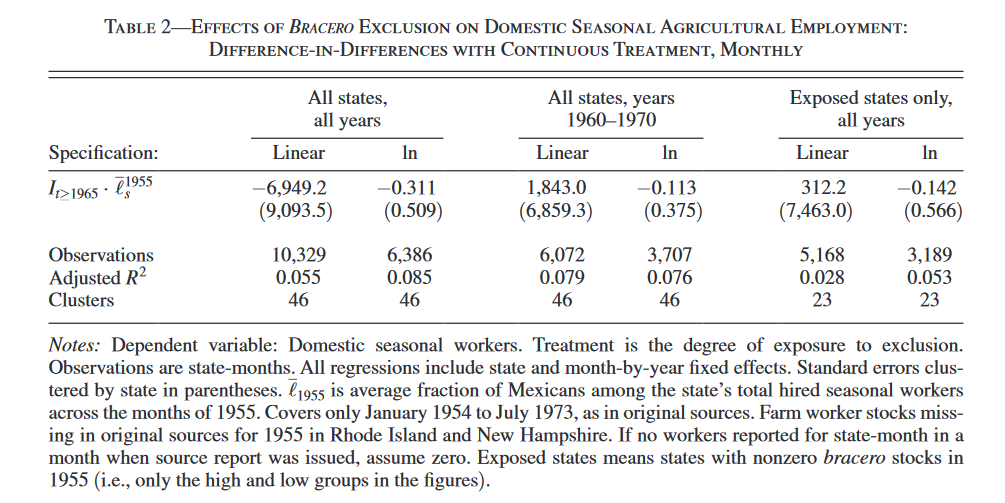
\includegraphics[width = \linewidth]{0731sugiyama/Table2.png}
        \label{fig:my_label}
    \end{figure}
    First two columns use all data, while the second two columns restrict the window of analysis to ten years.The coefficient estimate are statistically indistinguishable from zero.  \\
    Similar results are obtained for local, intrastate, and interstate US workers separately (panel B of Figure 3 and Table 3). This indicate that domestic seasonal workers did not move within or between state insubstantial number to dissipate state-specific shocks to the bracero labor supply. 
    
    {\bf Robustness check} \\
    Authors conduct fixed effect regression to check robustness. Panel A of Figure 4 show a Baltagi-Li(2002) semiparametric of real wage on bracero stock by state-quarter, with state and quarter-by-year fixed effects.
    
    \begin{figure}
        \centering
        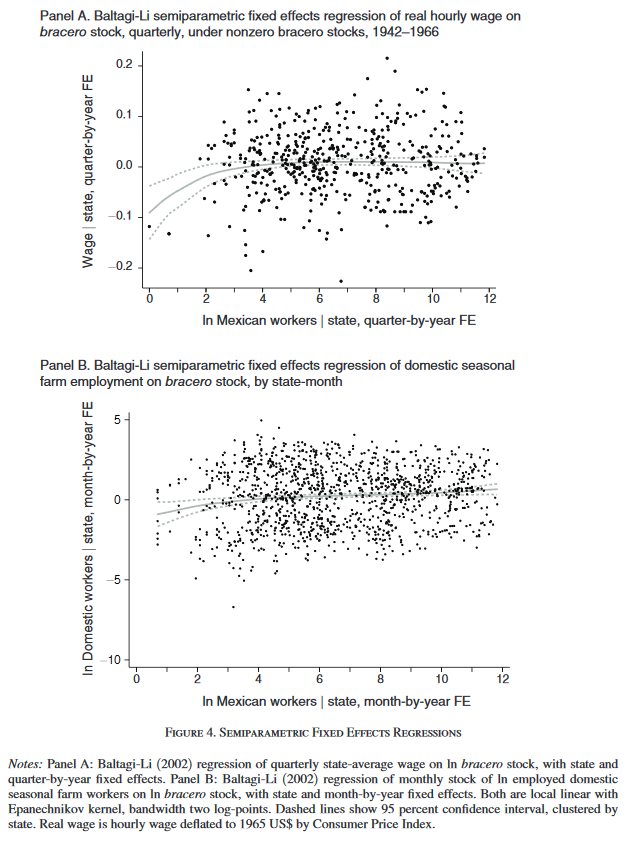
\includegraphics[width = \linewidth]{0731sugiyama/Figure4.png}
        \label{fig:my_label}
    \end{figure}
    Panel B shows the analogous semiparametric regression of domestic seasonal farm employment on bracero stock by state-month, with state and month-by-year fixed effect. \\
    These reveal no significant tendency for wages or domestic bracero stocks.
    
    
    {\bf Mechanism} \\
    These results imply that bracero exclusion failed as active labor market.
    The model predict this fail. Equation (6) and (7) suggest the policy's effect cause capital-labor substitution and technological adjustment. \\
    Panel A of Figure 5 shows that bracero exclusion was followed immediately by a dramatic adoption of this existing technology, as predicted by equation (7). 
    \begin{figure}
        \centering
        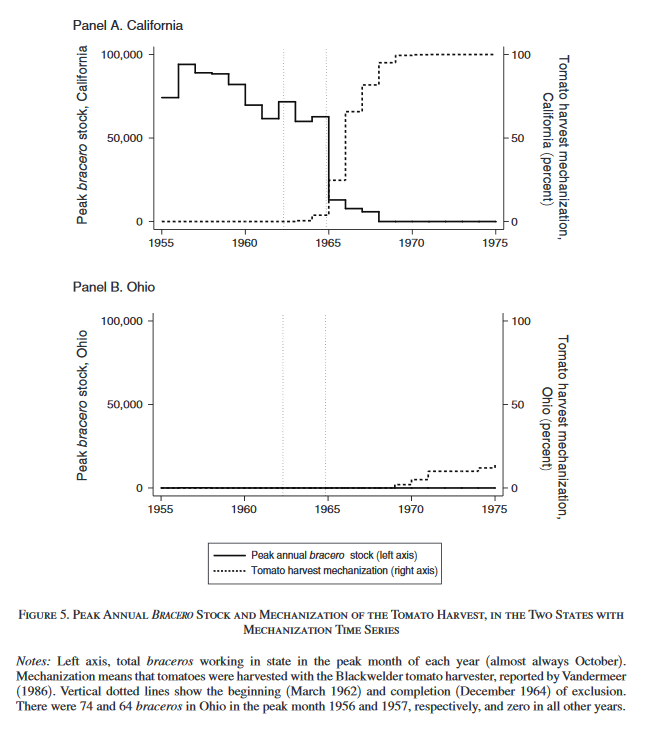
\includegraphics[width = \linewidth]{0731sugiyama/Figure5.png}
        \label{fig:my_label}
    \end{figure}
    Advanced mechanization technology was available for adoption to produce to tomatoes, cotton, and partially for sugar beets. \\
    No comparable technology was available for production of most of other crops. \\
    Authors expect greater reduction decline in production after exclusion for this latter group of crops.Authors test prediction with the event-study specification 
    \begin{align}
        y_{st} = \alpha' I_{s} + \beta'I_{t\neq 1964} +\gamma' \cdot I_{t\neq1964} \cdot \overline{l}^{1955} +\epsilon_{st} 
    \end{align}
    The outcome $y_{st}$ is a state- and crop-specific index of physical production(e.g.,ponds) scale to 100 in 1964. \\
    Figure 6 show the event-study coefficient estimate $\hat{\gamma}$ from equation (9) for nine of the most important bracero crops.  \\
    At the tomatoes and cottons on the figure, bracero exclusion is followed modest. \\
    
    \begin{figure}
        \centering
        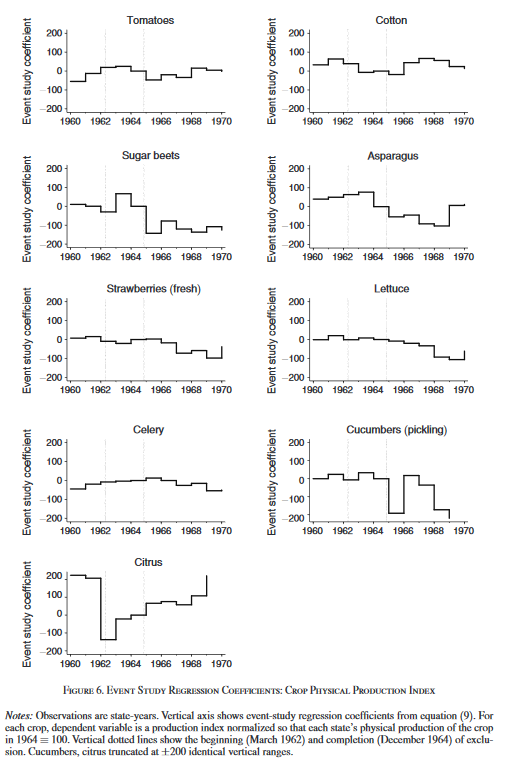
\includegraphics[width = \linewidth]{0731sugiyama/Figure6.png}
        \label{fig:my_label}
    \end{figure}
    For sugar beets, where adoption advanced technology faced greater friction, the relative decline after exclusion is larger and longer. \\
    Of the remaining six corps, where capital-labor could largely proceed only under the old technology, large and lasting relative decline is observed in production in and after 1965 in five.  \\
    An important concern is the potential for reverse causation of bracero exclusion by technical advance.Agribusiness lobbyists in bracero states could have stopped supporting the program precise when exogenous technical advance had reduced their need for labor.  But Congressional voting data collected by Alston and Ferrie (2007) show that no such shift occurred.
    
     {\bf Pre-trends} \\
    Authors explore the possibility of bias of bias from pre-trends in three ways:  
    \begin{itemize}
        \item Recasting the regressions year-by-year event-study
        \item Graphic the raw employment data for high-exposure states
        \item Running the core regression from above regression with added state-specific time-trends
    \end{itemize}
    Figure A1 show the core regression with real hourly wage as the outcomes. reformulated as year-by-year event study. No confounding pre-trend is evident; if anything, the wage gap between high-exposure and low-exposure was rising before exclusion, which would tend to bias the results towards finding a positive impact of exclusion on wages.    
    \begin{figure}
        \centering
        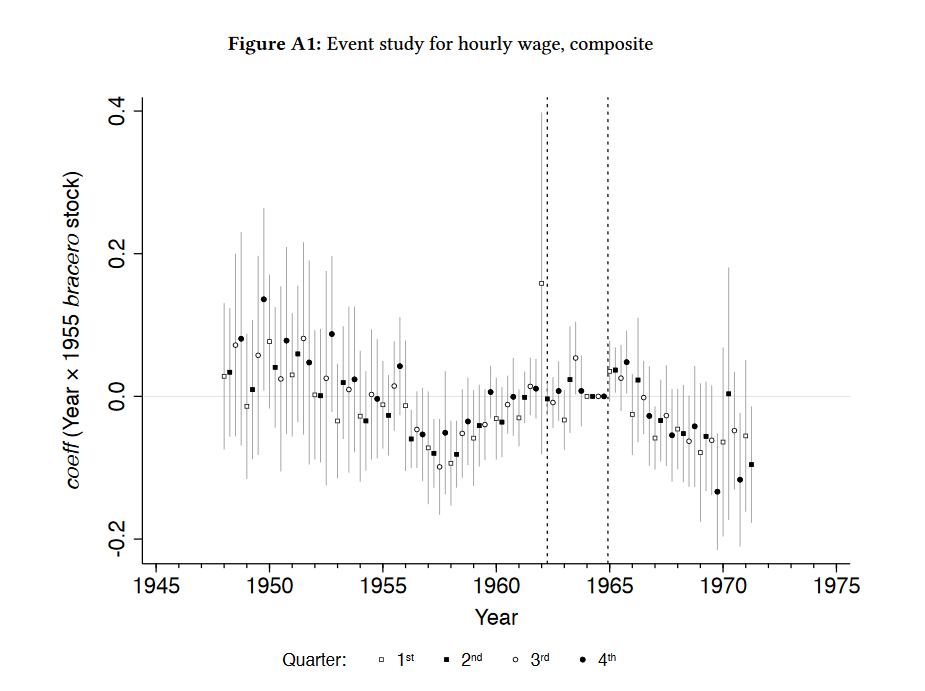
\includegraphics[width = \linewidth]{0731sugiyama/FigureA1.png}
        \label{fig:my_label}
    \end{figure}
    
    Figure 2 show similar exercise where the outcome is domestic hired seasonal workers in each state-month. \\
    There is a clear and statistically significant pre-tends in the late-season(September) to illustrate.This bias potentially confounding because such trends would bias downward any positive impact of exclusion on downward any positive impact of exclusion on domestic employment measure by DID. \\
    This pre-trends is limited to state with zero exposure to exclusion. If authors restrict the sample to states that had a nonzero number of bracero in 1955 (Figure A2b), there is no longer statistically significant pre-trends in either early- or late season month prior exclusion. \\
    Figure 3 show the raw employment data for the nine highest-exposure states.
    
    Domestic hired seasonal farm employment in each state-month is shown by black line, bracero by the gray line. Authors check whether the width of the domestic-Mexican employment gaps were changed before- and after- exclusion.     
    \begin{figure}
        \centering
        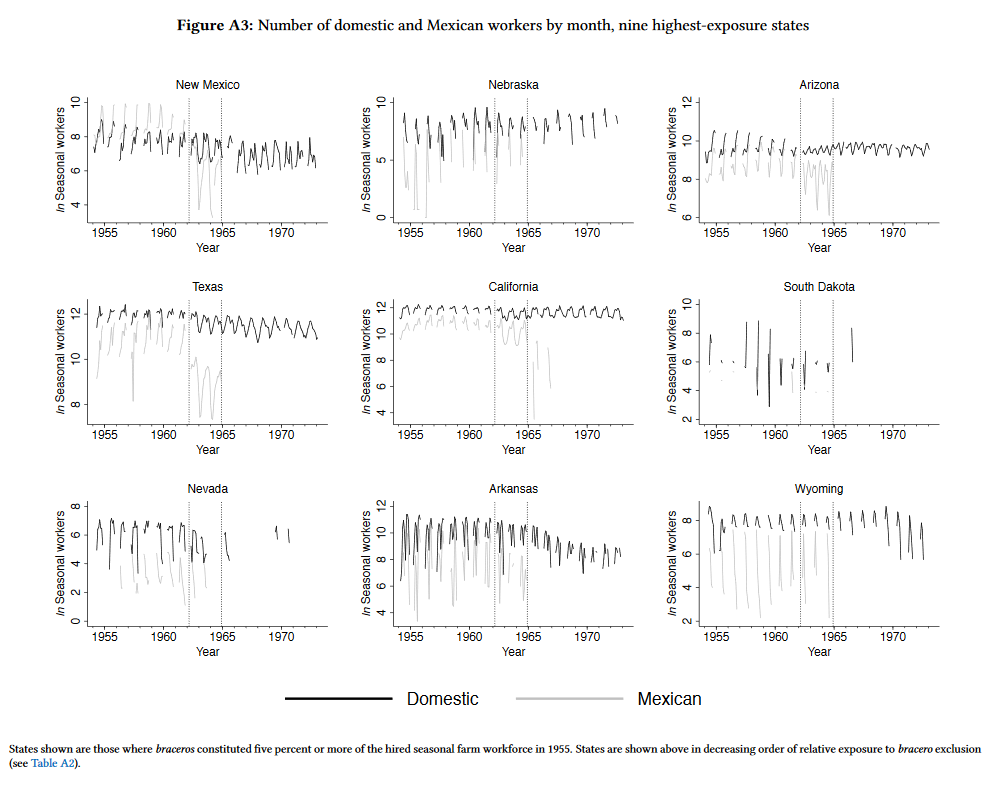
\includegraphics[width = \linewidth]{0731sugiyama/FigureA3.png}
        \label{fig:my_label}
    \end{figure}
    Authors conduct re-DID regression adding state specific linear time trends.
    
    \begin{align*}
         y_{st}= \alpha' I_s + \beta'I_t +\gamma(I_{t \geq 1965} \cdot \overline{l}^{1955}_s) +\xi'I_s \cdot t' \epsilon,
    \end{align*}
    where $\xi'I_s$ is a state-specific slope on the year $t'$.
    The results is that coefficient is shift but insignificant. Table A5 and A6 show the results.
    \begin{figure}
        \centering
        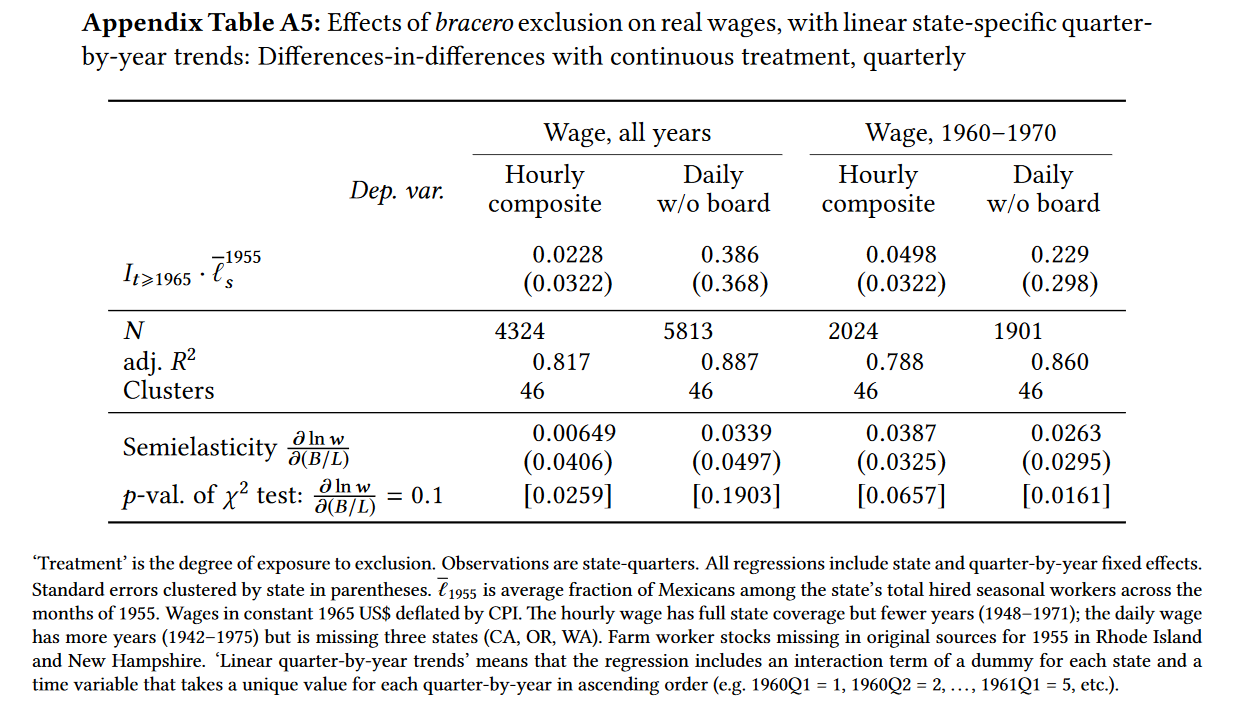
\includegraphics[width = \linewidth]{0731sugiyama/TableA5.png}
        \label{fig:my_label}
    \end{figure}
    \begin{figure}
        \centering
        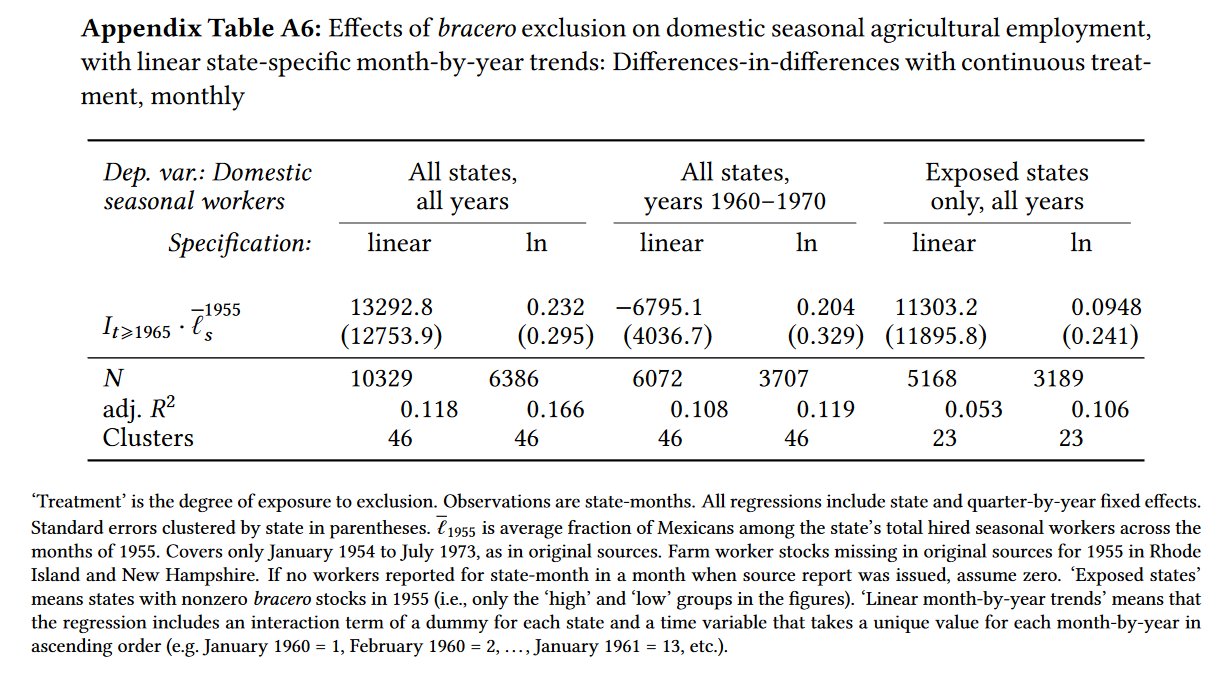
\includegraphics[width = \linewidth]{0731sugiyama/TableA6.png} 
        \label{fig:my_label}
    \end{figure}
    \section{Conclusion}
    \begin{itemize}
        \item Bracero exclusion failed to substantially raise wages or employment for domestic workers in the sector.
        \item Employment appear to have instead adjusted to foreign-worker exclusion by changing protection technology, where was possible, and changing production levels where it was not.
        \item Further research should explore other natural experiments to test causal links between labor scarcity and endogenous technical changes, as urged Acemoglu (2010).  
    \end{itemize}
      
    
    
    \biblio
    
\end{document}